\section{Our Approach}
\label{sec:ourApproach}

In this section, we introduce our approach and explain the technical challenges involved in realizing it in a manner that is both secure and easy to deploy. 

\subsection{Input Trace Matching}

We propose a conceptually simple approach for the protection of user input integrity that we call \emph{input trace matching}. Our approach is tailored for keyboard input that is delivered to a remote server through a web application running on an untrusted host, as illustrated in Figure~\ref{fig:abstractModel}. 

\begin{figure}[t]
 \centering
  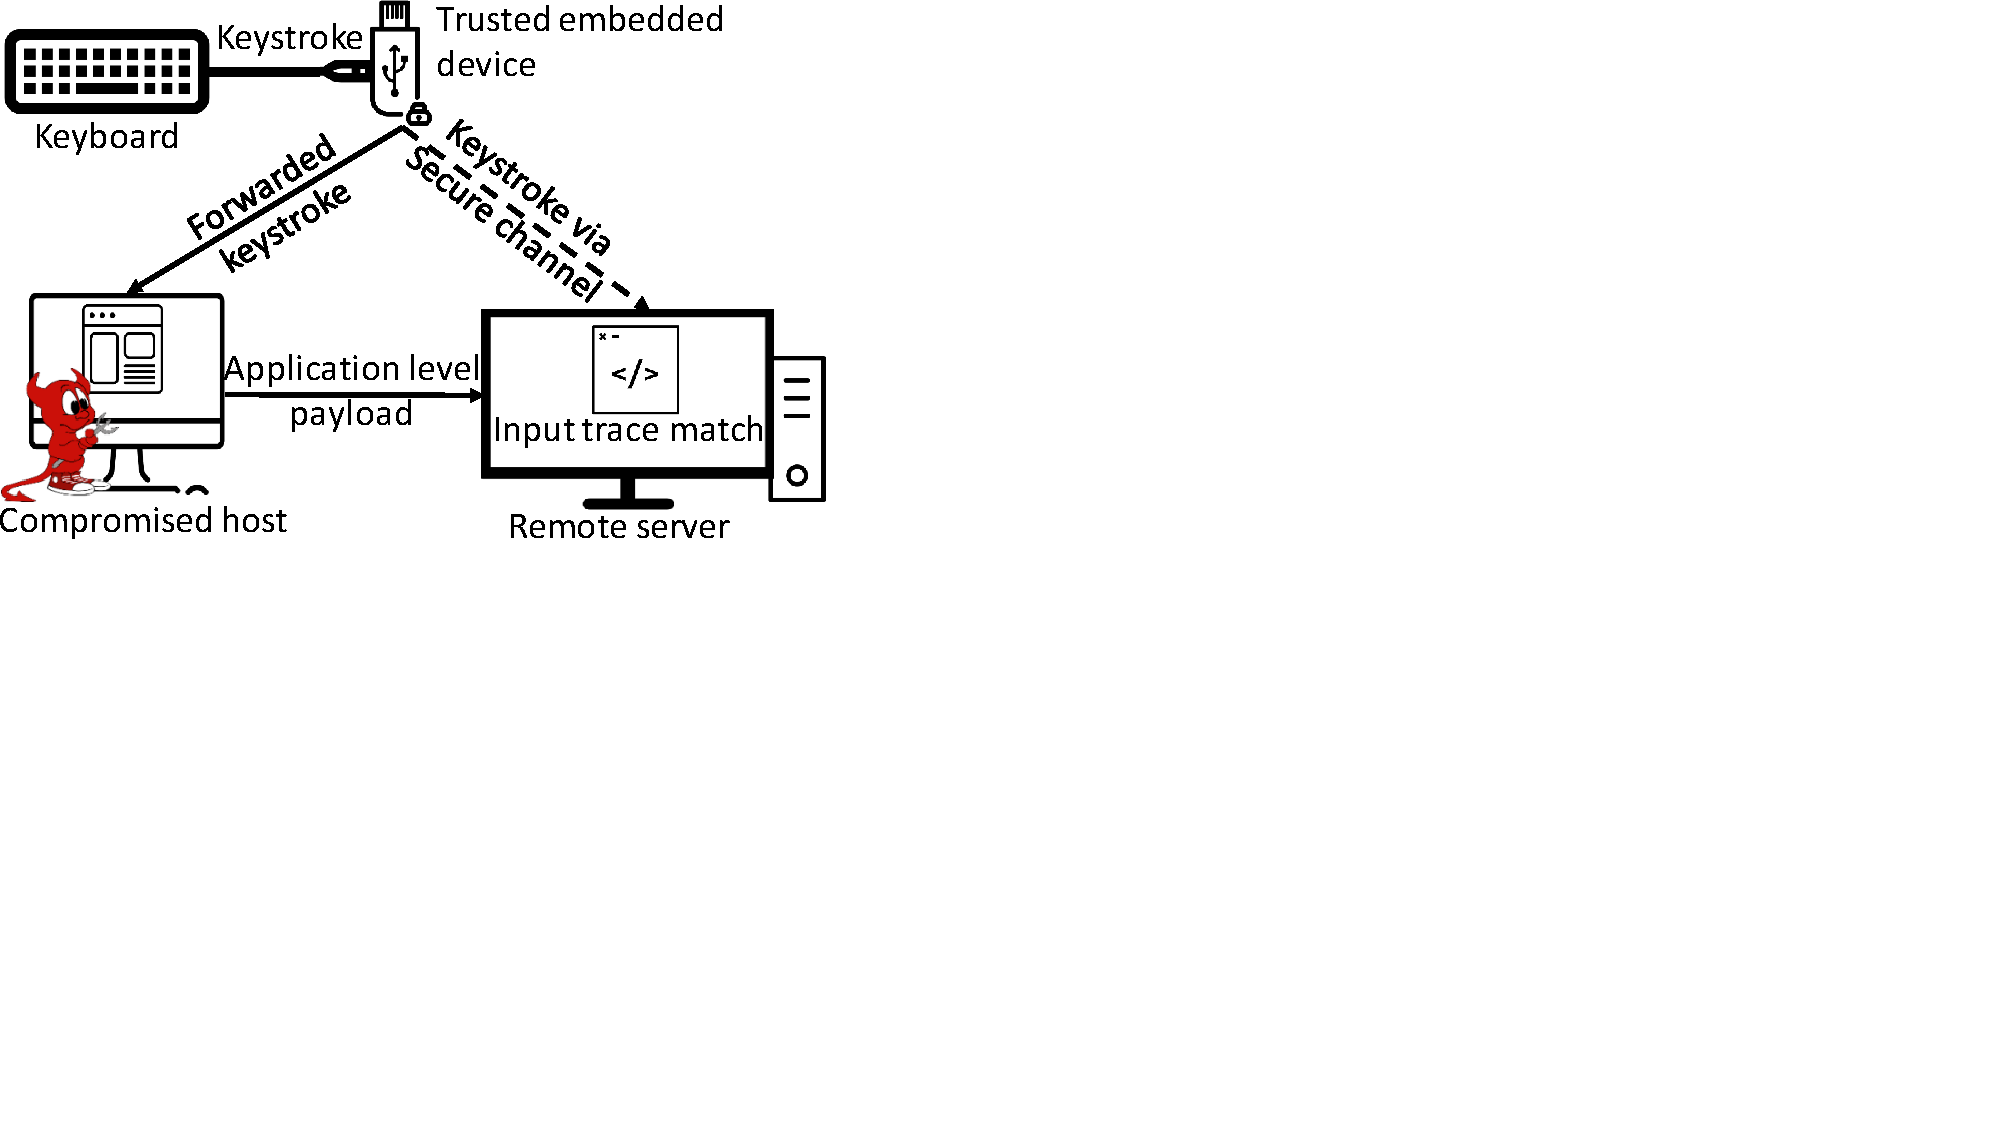
\includegraphics[trim={0 9cm 19.5cm 0},clip,width=0.7\linewidth]{chapters/IntegriKey/images/AbstractModel.pdf}
 \caption[Approach overview]{\textbf{Approach overview.} The user connects a trusted embedded device between the host and the keyboard. This device relays received keystroke events to the host and sends a trace of them over a secure channel to the remote server. The server compares the trace to the application payload received from the host to detect user input manipulation.}
 
 \label{fig:abstractModel}
\end{figure}

The main component of the solution is a trusted embedded device. When the user needs to perform a security-critical web transaction like configuring a PLC or performing a cryptocurrency transaction, the user connects the embedded device \emph{between} the keyboard and the host. The connection from the keyboard to the embedded device and from the embedded device to the host can be wired (e.g., USB) or wireless (e.g., Bluetooth). We consider the embedded device trusted because it performs only very limited functionality and therefore it has significantly smaller software TCB, attack surface and hardware complexity compared to the host. 

The trusted embedded device performs two types of functionalities. The first functionality is that it forwards received keystroke events from the keyboard to the host. The application running on the host (e.g., a web browser) receives the user input events and constructs an application-level payload (e.g., an HTTP response) that it sends to the server. Our approach imposes no changes to the host platform or the application software running on it. The second functionality of the embedded device is that it sends a trace of the intercepted keystrokes to an authenticated and authorized remote server over a secure channel when the user either changes the text field (by pressing tab key) or submits the form (by pressing an enter key).

The server parses the application payload received from the host and extracts the user input values from it. Then it compares input values to the received traces to detect any possible discrepancies. If the input values and keystroke events in the traces match, the user input can be safely accepted.

Once the user has completed the web transaction, he can remove the embedded device from between the host and the keyboard. This action prevent further input events from being forwarded to the server. Therefore, our solution does not violate user's privacy by exposing user's input outside the security-critical task to the authorized server. We discuss user privacy in more detail in Section~\ref{sec:privacy}.

\subsection{Challenges}
\label{sec:ourApproach:challenges}

Realizing the above idea involves both security and deployment challenges that we discuss next.

\myparagraph{Swapping attacks} Input trace matching, as outlined above, prevents \emph{most} user input manipulations by the untrusted host. For example, if the user types in one value, but the application payload contains another, the server can detect the mismatch and abort the operation. 

However, the adversary may still perform more subtle and \emph{restricted} forms of user input manipulation.
The problem is exemplified by our running example UI, shown in Figure~\ref{fig:swapExample}. Input trace matching allows the server to verify that all values received from the host were indeed typed in by the user, but since some values may \emph{interchangeable} (i.e., they can have the same format and overlapping acceptable ranges), the untrusted host can perform a user input manipulation that we identify and call as \emph{swapping attack}.

\begin{figure}[t]
  \centering

     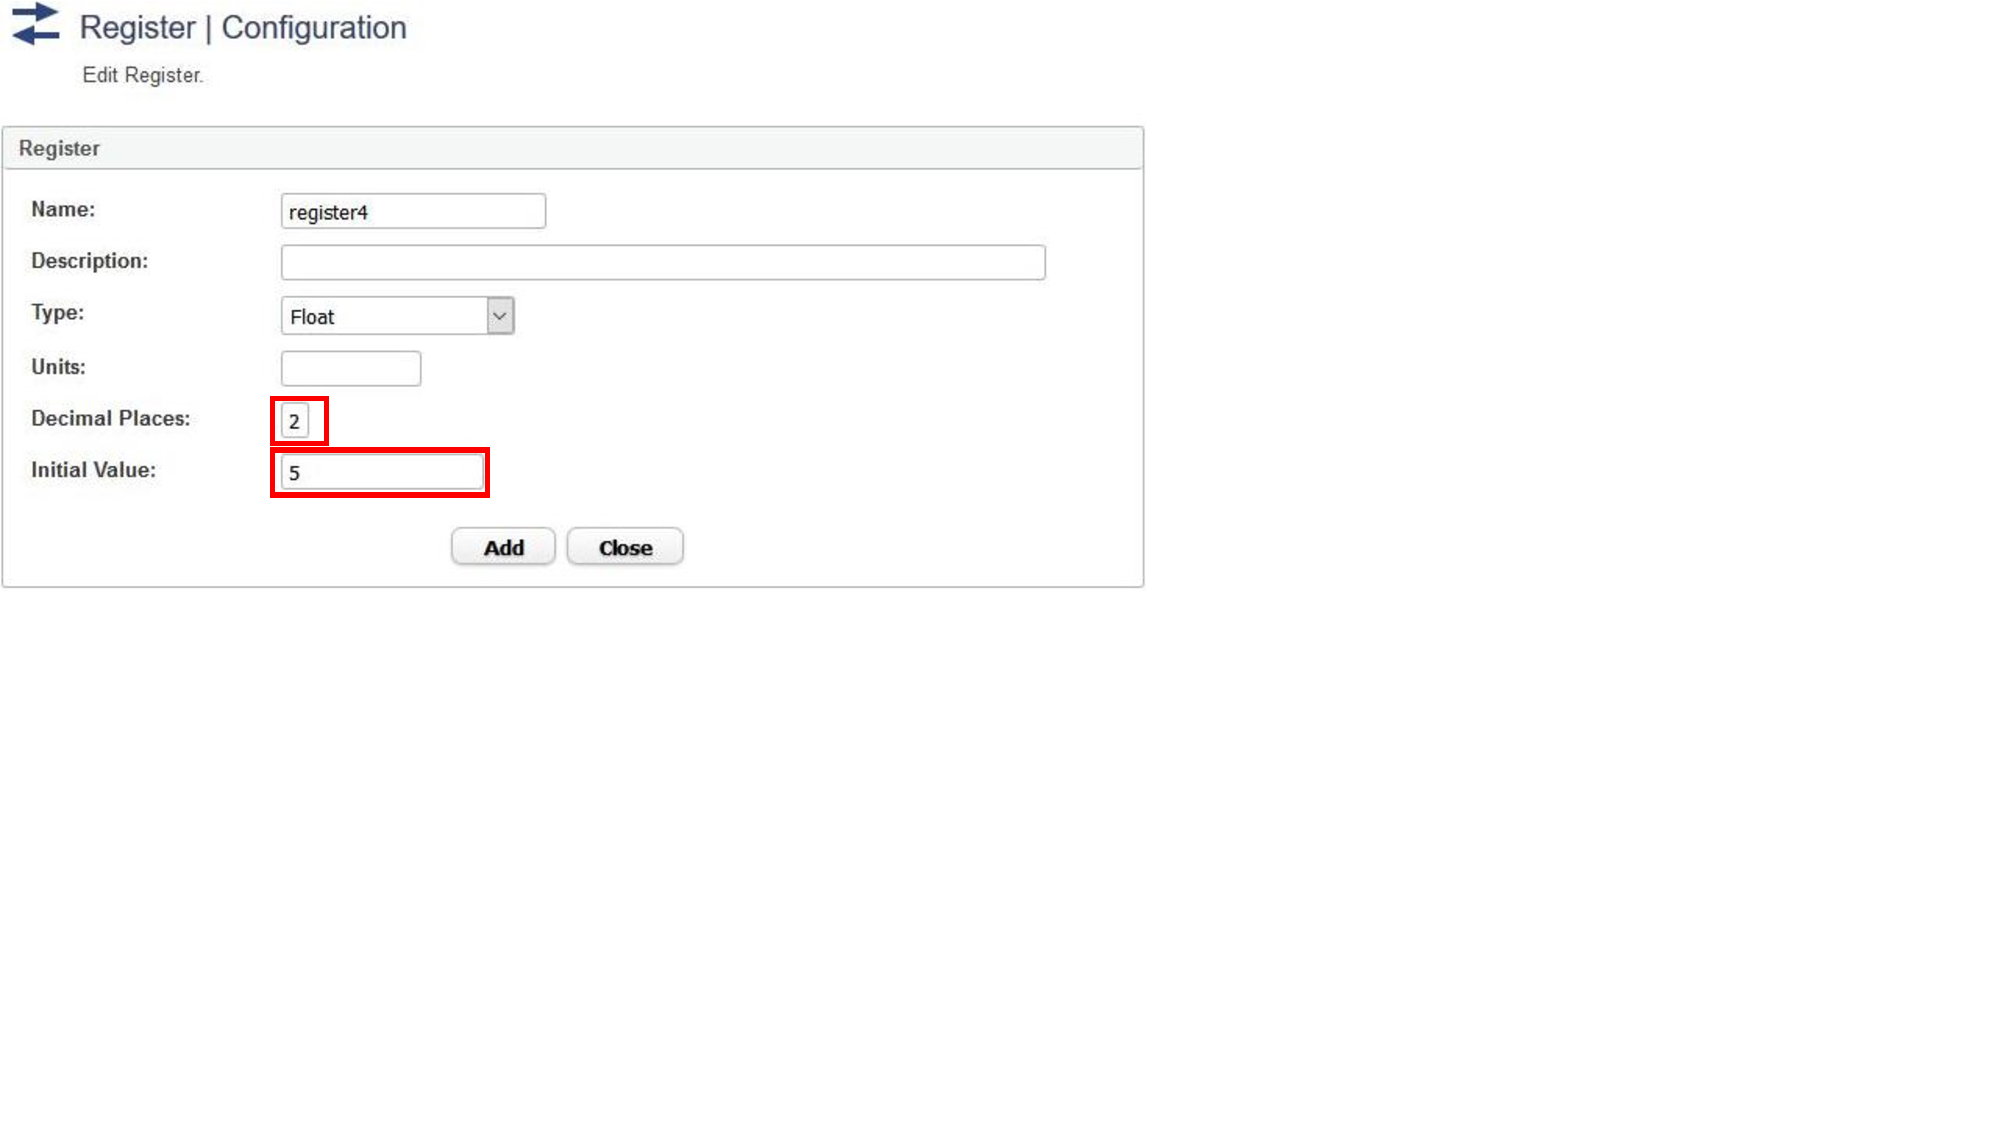
\includegraphics[trim={0 -1cm 14cm 0},clip, width=0.65\linewidth]{chapters/IntegriKey/images/SwapExample.pdf}
    \caption[Swapping attack and interchangeable inputs]{\textbf{Swapping attack and interchangeable inputs.} This screenshot shows our running example UI (PLC configuration web form), where the `\texttt{Relay temp 1}' and `\texttt{Relay temp 2}' user input field descriptions in the UI are swapped by the adversary. The corresponding HTTP response packet shows the swapped value of these two fields. Additionally, the figures shows groups of input fields that are swappable.} 
    \label{fig:swapExample} 
\end{figure}


In a swapping attack, the malicious host manipulates the web form that is shown to the user and the application payload that is sent to the server. Figure~\ref{fig:swapExample} illustrates one such example, where the malicious host swaps the field names '\texttt{Relay temp1}' and '\texttt{Relay temp2}' in the UI. The user is likely to enter the values based on the swapped field names, but the server will interpret the user input differently, based on the manipulated HTTP response constructed by the host, as shown in Figure~\ref{fig:swapExample}. Because the order of the user input in the received trace matches the HTTP response, the server cannot detect such manipulation from the input order. Assuming that the entered values are in the overlapping region of acceptable values for the respective input fields, the server cannot detect such manipulation based on the received values either. 

Similarly, the adversary can swap any interchangeable user input fields (overlapping format and range) in the UI. Figure~\ref{fig:swapExample} shows a grouping for all interchangeable values in our example web form.

%One example is in the home automation system, the user can set the temperature of a specific room by providing the input to the web application. The attacker can swap the labels of the field with the label of the temperature of another room. More interesting examples are the fields which are semantically disjoint but share specifications. E.g., the parameters for the medical devices where the doctor can set `blood pressure' and `heart rate limit'. As the range of these two fields is overlapping, the attacker can swap the labels of two such fields even though the fields `blood pressure' and `heart rate limit' are semantically different. 

\myparagraph{Adoption challenges} Input trace matching requires a secure communication channel from the trusted embedded device to the server. Our goal is to keep the device simple (small TCB) and inexpensive, and thus we avoid designs where the embedded device has its own communication capabilities (e.g., dedicated cellular radio). Host-assisted communication requires installation of new software on the host which can complicate adoption and in some cases may not even be possible for the user. Ideally, connecting the trusted embedded device to the host should be all the user has to do.

Another adoption challenge is that a single device should be able to provide user input integrity protection for multiple web services. The device can be configured with the keys and addresses of all supported servers, but during deployment, we want to avoid additional user tasks, such as manually indicating which of the pre-configured servers should be used.


